%4619055 課題3 パルス回路
\documentclass[12pt]{jarticle}
\usepackage{TUSIreport}
\usepackage{otf}
\usepackage[dvipdfmx]{graphicx}
\usepackage{amsmath}
\usepackage{amssymb}
\usepackage{hhline}
\usepackage{fancybox,ascmac}
\usepackage{url}
%%%%%%%%%%%%%%%%%%
\begin{document}
%%%%%%%%%%%%%%%%%%%%%%%%%%%%%%%%%%%%%%%%%%%%%%%%%%%%%%%%
% 表紙を出力する場合は,\提出者と\共同実験者をいれる
% \提出者{科目名}{課題名}{提出年}{提出月}{提出日}{学籍番号}{氏名}
% \共同実験者{一人目}{二人目}{..}{..}{..}{..}{..}{八人目}
%%%%%%%%%%%%%%%%%%%%%%%%%%%%%%%%%%%%%%%%%%%%%%%%%%%%%%%
\提出者{情報工学実験1}{課題4 }
{2020}{7}{27}{4619055}{辰川力駆}

\共同実験者{}{}{}{}{}{}{}{}
\追加実験者{}{}
\表紙出力

\section{実験の目的}
実験を通して、誤差を体感し、データを視覚的に表現する。
指標

\section{実験1}
サイコロを用いたギャンブル

\subsection{目標}
\begin{itemize}
    \item 実験を通して実際にデータがばらつくことを実感する
    \item 簡単なギャンブルを例に、誤差について考える
\end{itemize}
\subsection{実験手順}
\begin{itemize}
    \item[(1)] 1回の試行でサイコロ(出る目は0から9)を2個同時に振り、
          出た目の合計で以下のように収支が決まるギャンブルを考える
          \begin{itemize}
              \item 合計が7以下・・・1000円払う
              \item 合計が12以上・・・1500円もらう
              \item それ以外・・・引き分け
          \end{itemize}
    \item[(2)] 試行を100回繰り返し、各試行の目の合計・収支を記録する
    \item[(3)] 試行回数5回ごとに、1回目からの平均収支を求める。
    \item[(4)] 横軸に試行回数、縦軸に1回目からの平均収支をとり、
          平均収支が収束する様子をグラフで表現する(期待収支も記入)
\end{itemize}
\subsection{実験結果と考察}
以下にサイコロを100回振った結果と、サイコロを用いたギャンブルによる平均収支のグラフを示す。

\clearpage
\begin{table}
    \caption{サイコロを用いたギャンブルの記録}
    \begin{tabular}[h]{|r|c|c|c|c|c|c|}
        \hline
        試行回数 & サイコロ1の目 & サイコロ2の目 & 出た目の合計 & 収支  & 試行回数 & 平均収支     \\ \hline
        1        & 6             & 9             & 15           & 1500  &          &              \\
        2        & 8             & 7             & 15           & 1500  &          &              \\
        3        & 0             & 5             & 5            & -1000 & 5        & 200          \\
        4        & 4             & 6             & 10           & 0     &          &              \\
        5        & 7             & 0             & 7            & -1000 &          &              \\
        \hline6  & 6             & 3             & 9            & 0     &          &              \\
        7        & 5             & 2             & 7            & -1000 &          &              \\
        8        & 2             & 6             & 8            & 0     & 10       & 150          \\
        9        & 8             & 2             & 10           & 0     &          &              \\
        10       & 8             & 5             & 13           & 1500  &          &              \\
        \hline11 & 0             & 8             & 8            & 0     &          &              \\
        12       & 9             & 6             & 15           & 1500  &          &              \\
        13       & 4             & 6             & 10           & 0     & 15       & 66.66666667  \\
        14       & 5             & 1             & 6            & -1000 &          &              \\
        15       & 2             & 0             & 2            & -1000 &          &              \\
        \hline16 & 1             & 2             & 3            & -1000 &          &              \\
        17       & 9             & 1             & 10           & 0     &          &              \\
        18       & 7             & 3             & 10           & 0     & 20       & 0            \\
        19       & 4             & 6             & 10           & 0     &          &              \\
        20       & 0             & 9             & 9            & 0     &          &              \\
        \hline21 & 7             & 9             & 16           & 1500  &          &              \\
        22       & 4             & 1             & 5            & -1000 &          &              \\
        23       & 1             & 4             & 5            & -1000 & 25       & -20          \\
        24       & 7             & 1             & 8            & 0     &          &              \\
        25       & 4             & 6             & 10           & 0     &          &              \\
        \hline26 & 3             & 4             & 7            & -1000 &          &              \\
        27       & 2             & 9             & 11           & 0     &          &              \\
        28       & 6             & 1             & 7            & -1000 & 30       & -66.66666667 \\
        29       & 3             & 9             & 12           & 1500  &          &              \\
        30       & 6             & 0             & 6            & -1000 &          &              \\
        \hline31 & 5             & 9             & 14           & 1500  &          &              \\
        32       & 7             & 6             & 13           & 1500  &          &              \\
        33       & 4             & 6             & 10           & 0     & 35       & 71.42857143  \\
        34       & 8             & 6             & 14           & 1500  &          &              \\
        35       & 3             & 8             & 11           & 0     &          &              \\
        \hline36 & 6             & 6             & 12           & 1500  &          &              \\
        37       & 5             & 6             & 11           & 0     &          &              \\
        38       & 0             & 7             & 7            & -1000 & 40       & 50           \\
        39       & 8             & 0             & 8            & 0     &          &              \\
        40       & 6             & 1             & 7            & -1000 &          &              \\
        \hline
    \end{tabular}
\end{table}
\clearpage
\begin{table}
    \begin{tabular}[h]{|r|c|c|c|c|c|c|}
        \hline
        試行回数  & サイコロ1の目 & サイコロ2の目 & 出た目の合計 & 収支  & 試行回数 & 平均収支    \\ \hline
        41        & 9             & 0             & 9            & 0     &          &             \\
        42        & 7             & 2             & 9            & 0     &          &             \\
        43        & 7             & 4             & 11           & 0     & 45       & 77.77777778 \\
        44        & 8             & 9             & 17           & 1500  &          &             \\
        45        & 2             & 8             & 10           & 0     &          &             \\
        \hline 46 & 4             & 2             & 6            & -1000 &          &             \\
        47        & 5             & 4             & 9            & 0     &          &             \\
        48        & 3             & 9             & 12           & 1500  & 50       & 80          \\
        49        & 3             & 5             & 8            & 0     &          &             \\
        50        & 8             & 2             & 10           & 0     &          &             \\
        \hline 51 & 1             & 1             & 2            & -1000 &          &             \\
        52        & 9             & 4             & 13           & 1500  &          &             \\
        53        & 9             & 8             & 17           & 1500  & 55       & 109.0909091 \\
        54        & 4             & 5             & 9            & 0     &          &             \\
        55        & 1             & 7             & 8            & 0     &          &             \\
        \hline 56 & 0             & 3             & 3            & -1000 &          &             \\
        57        & 9             & 3             & 12           & 1500  &          &             \\
        58        & 1             & 3             & 4            & -1000 & 60       & 91.66666667 \\
        59        & 4             & 6             & 10           & 0     &          &             \\
        60        & 5             & 6             & 11           & 0     &          &             \\
        \hline 61 & 0             & 0             & 0            & -1000 &          &             \\
        62        & 1             & 2             & 3            & -1000 &          &             \\
        63        & 5             & 3             & 8            & 0     & 65       & 23.07692308 \\
        64        & 4             & 0             & 4            & -1000 &          &             \\
        65        & 6             & 0             & 6            & -1000 &          &             \\
        \hline66  & 3             & 8             & 11           & 0     &          &             \\
        67        & 8             & 2             & 10           & 0     &          &             \\
        68        & 7             & 8             & 15           & 1500  & 70       & 28.57142857 \\
        69        & 8             & 1             & 9            & 0     &          &             \\
        70        & 3             & 1             & 4            & -1000 &          &             \\
        \hline71  & 7             & 4             & 11           & 0     &          &             \\
        72        & 3             & 2             & 5            & -1000 &          &             \\
        73        & 2             & 3             & 5            & -1000 & 75       & 20          \\
        74        & 9             & 8             & 17           & 1500  &          &             \\
        75        & 6             & 5             & 11           & 0     &          &             \\
        \hline76  & 5             & 2             & 7            & -1000 &          &             \\
        77        & 6             & 7             & 13           & 1500  &          &             \\
        78        & 0             & 1             & 1            & -1000 & 80       & -12.5       \\
        79        & 4             & 0             & 4            & -1000 &          &             \\
        80        & 1             & 1             & 2            & -1000 &          &             \\
        \hline
    \end{tabular}
\end{table}
\clearpage
\begin{table}
    \begin{tabular}[h]{|r|c|c|c|c|c|c|}
        \hline
        試行回数 & サイコロ1の目 & サイコロ2の目 & 出た目の合計 & 収支  & 試行回数 & 平均収支     \\
        \hline
        81       & 6             & 5             & 11           & 0     &          &              \\
        82       & 4             & 6             & 10           & 0     &          &              \\
        83       & 3             & 3             & 6            & -1000 & 85       & -5.882352941 \\
        84       & 2             & 6             & 8            & 0     &          &              \\
        85       & 5             & 7             & 12           & 1500  &          &              \\
        \hline
        86       & 4             & 3             & 7            & -1000 &          &              \\
        87       & 9             & 0             & 9            & 0     &          &              \\
        88       & 4             & 8             & 12           & 1500  & 90       & -22.22222222 \\
        89       & 0             & 0             & 0            & -1000 &          &              \\
        90       & 0             & 6             & 6            & -1000 &          &              \\
        \hline
        91       & 4             & 8             & 12           & 1500  &          &              \\
        92       & 7             & 5             & 12           & 1500  &          &              \\
        93       & 2             & 8             & 10           & 0     & 95       & -10.52631579 \\
        94       & 0             & 6             & 6            & -1000 &          &              \\
        95       & 3             & 4             & 7            & -1000 &          &              \\
        \hline
        96       & 0             & 9             & 9            & 0     &          &              \\
        97       & 3             & 1             & 4            & -1000 &          &              \\
        98       & 7             & 8             & 15           & 1500  & 100      & -15          \\
        99       & 1             & 0             & 1            & -1000 &          &              \\
        100      & 7             & 2             & 9            & 0     &          &              \\
        \hline
    \end{tabular}
\end{table}
\begin{figure}[h]
    \begin{center}
        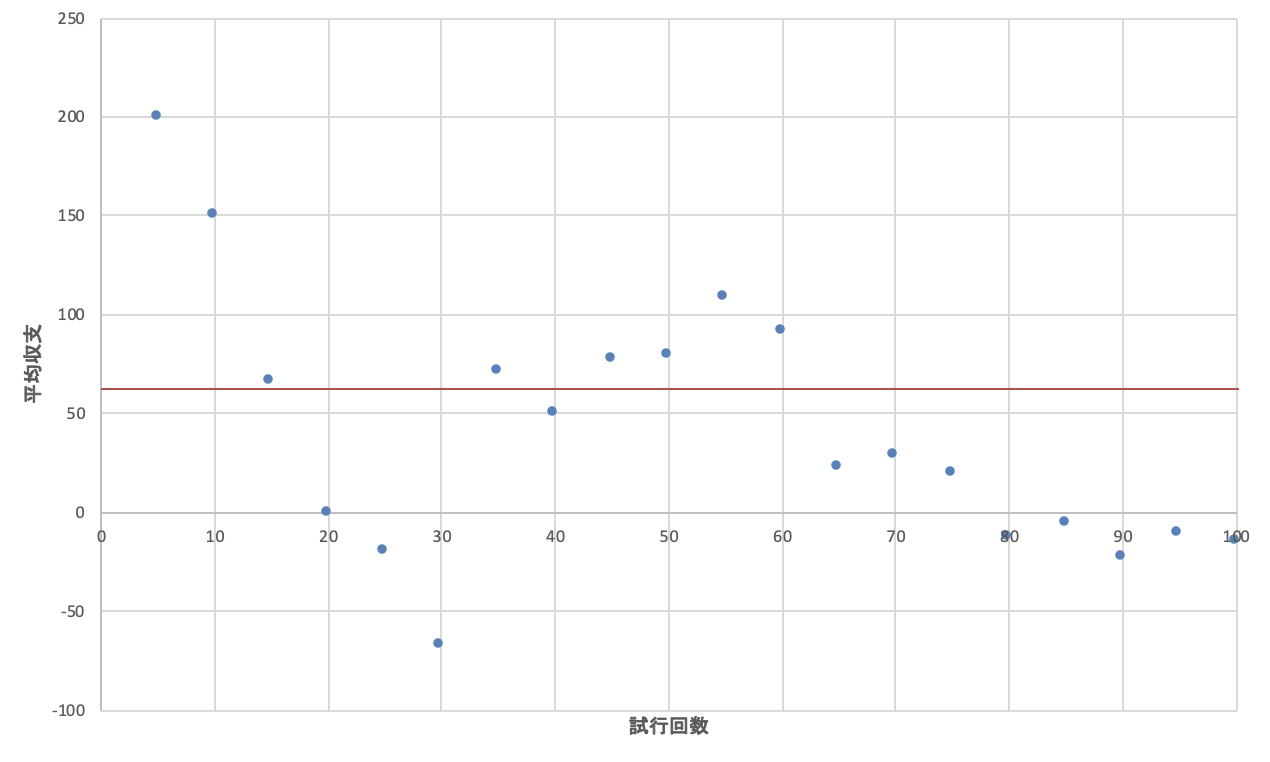
\includegraphics[scale=0.8]{kadai4_graph1.png}
    \end{center}
    \caption{平均収支の変化}
    \label{fig1}
\end{figure}
\clearpage

また、図1の赤い直線は期待収支を表している。
求め方は、
\begin{eqnarray}
    E[Y] &=& \frac{36}{100}×(-1000) + \frac{28}{100}×1500 + \frac{36}{100}×0 \nonumber\\
    &=& 60
\end{eqnarray}
で求められる。

よって、1 回の収支の期待収支は 60 円と言うことが分かるので、$y(平均収支)=60$の直線を引いている。

\subsection{レポート課題}
\subsubsection*{レポート課題1-1}
\begin{shadebox}
    1回の試行における収支の期待値を計算し、
    5回の試行が終わったときの実験結果と比較せよ。
    さらに、100回の試行が終わったときの実験結果と比較せよ。
\end{shadebox}
式(1)より、1回の試行における収支の期待値は60円である。

5回の試行が終わったときの収支は表1より200円で、
1回の試行における収支の期待値との差は140円で差が大きかった。
試行回数が少ないとばらつきが大きくなってし
まうことがあると考えられる.
100 回の試行が終わったときの収支は表 1 より 35 円で,1 回の試行における期待値との差は
15 円となり,5 回の試行の結果よりはかなり差が狭まった.試行回数が増えるとばらつきが減っ
ていくことが分かった.

\subsubsection*{レポート課題1-2}
\begin{shadebox}
    出た目の合計Xのヒストグラムを作成し、
    ヒストグラムからわかることをまとめよ。
\end{shadebox}

\subsubsection*{レポート課題1-3}
\begin{shadebox}
    このギャンブルの1回の参加費が120円のとき、
    参加すべきかどうかを理由とともに説明せよ。
    また、サイコロの目が12以上のときに何円受け取ることができればよいか
    (すなわち、期待される収支が0円以上となるか)を述べよ。
\end{shadebox}

\section{実験2}

\subsection{目標}

\subsection{実験手順}
\subsection{実験結果と考察}
\subsection{レポート課題}
\subsubsection*{レポート課題2-1}
\begin{shadebox}
    実験2で扱ったデータを用いて2倍の区間幅(100万円刻み)を持つ
    ヒストグラムを作成せよ。
\end{shadebox}

\subsubsection*{レポート課題2-2}
\begin{shadebox}
    作成した2つのヒストグラムを比較し、
    視覚的に得られる情報にどのような違いがあるか考察せよ。
\end{shadebox}

\subsubsection*{レポート課題2-3}
\begin{shadebox}
    本データを要約する際に、平均値は適切であるといえるか、理由とともに述べよ。
\end{shadebox}

\subsubsection*{レポート課題2-4}
\begin{shadebox}
    ヒストグラムからわかることと、箱ひげ図からわかることの違いを述べよ。
    またそれはなぜかを述べよ。
    さらに、ヒストグラムよりも箱ひげ図を用いたほうが適切だと思われる例を挙げよ。
\end{shadebox}

\subsubsection*{レポート課題2-5}
\begin{shadebox}
    データを要約する指標を列挙し、それぞれの内容と特徴を述べよ。
\end{shadebox}

\subsection{双安定マルチバイブレータ(フリップフロップ)}

\clearpage
\begin{figure}[h]
    \begin{center}
        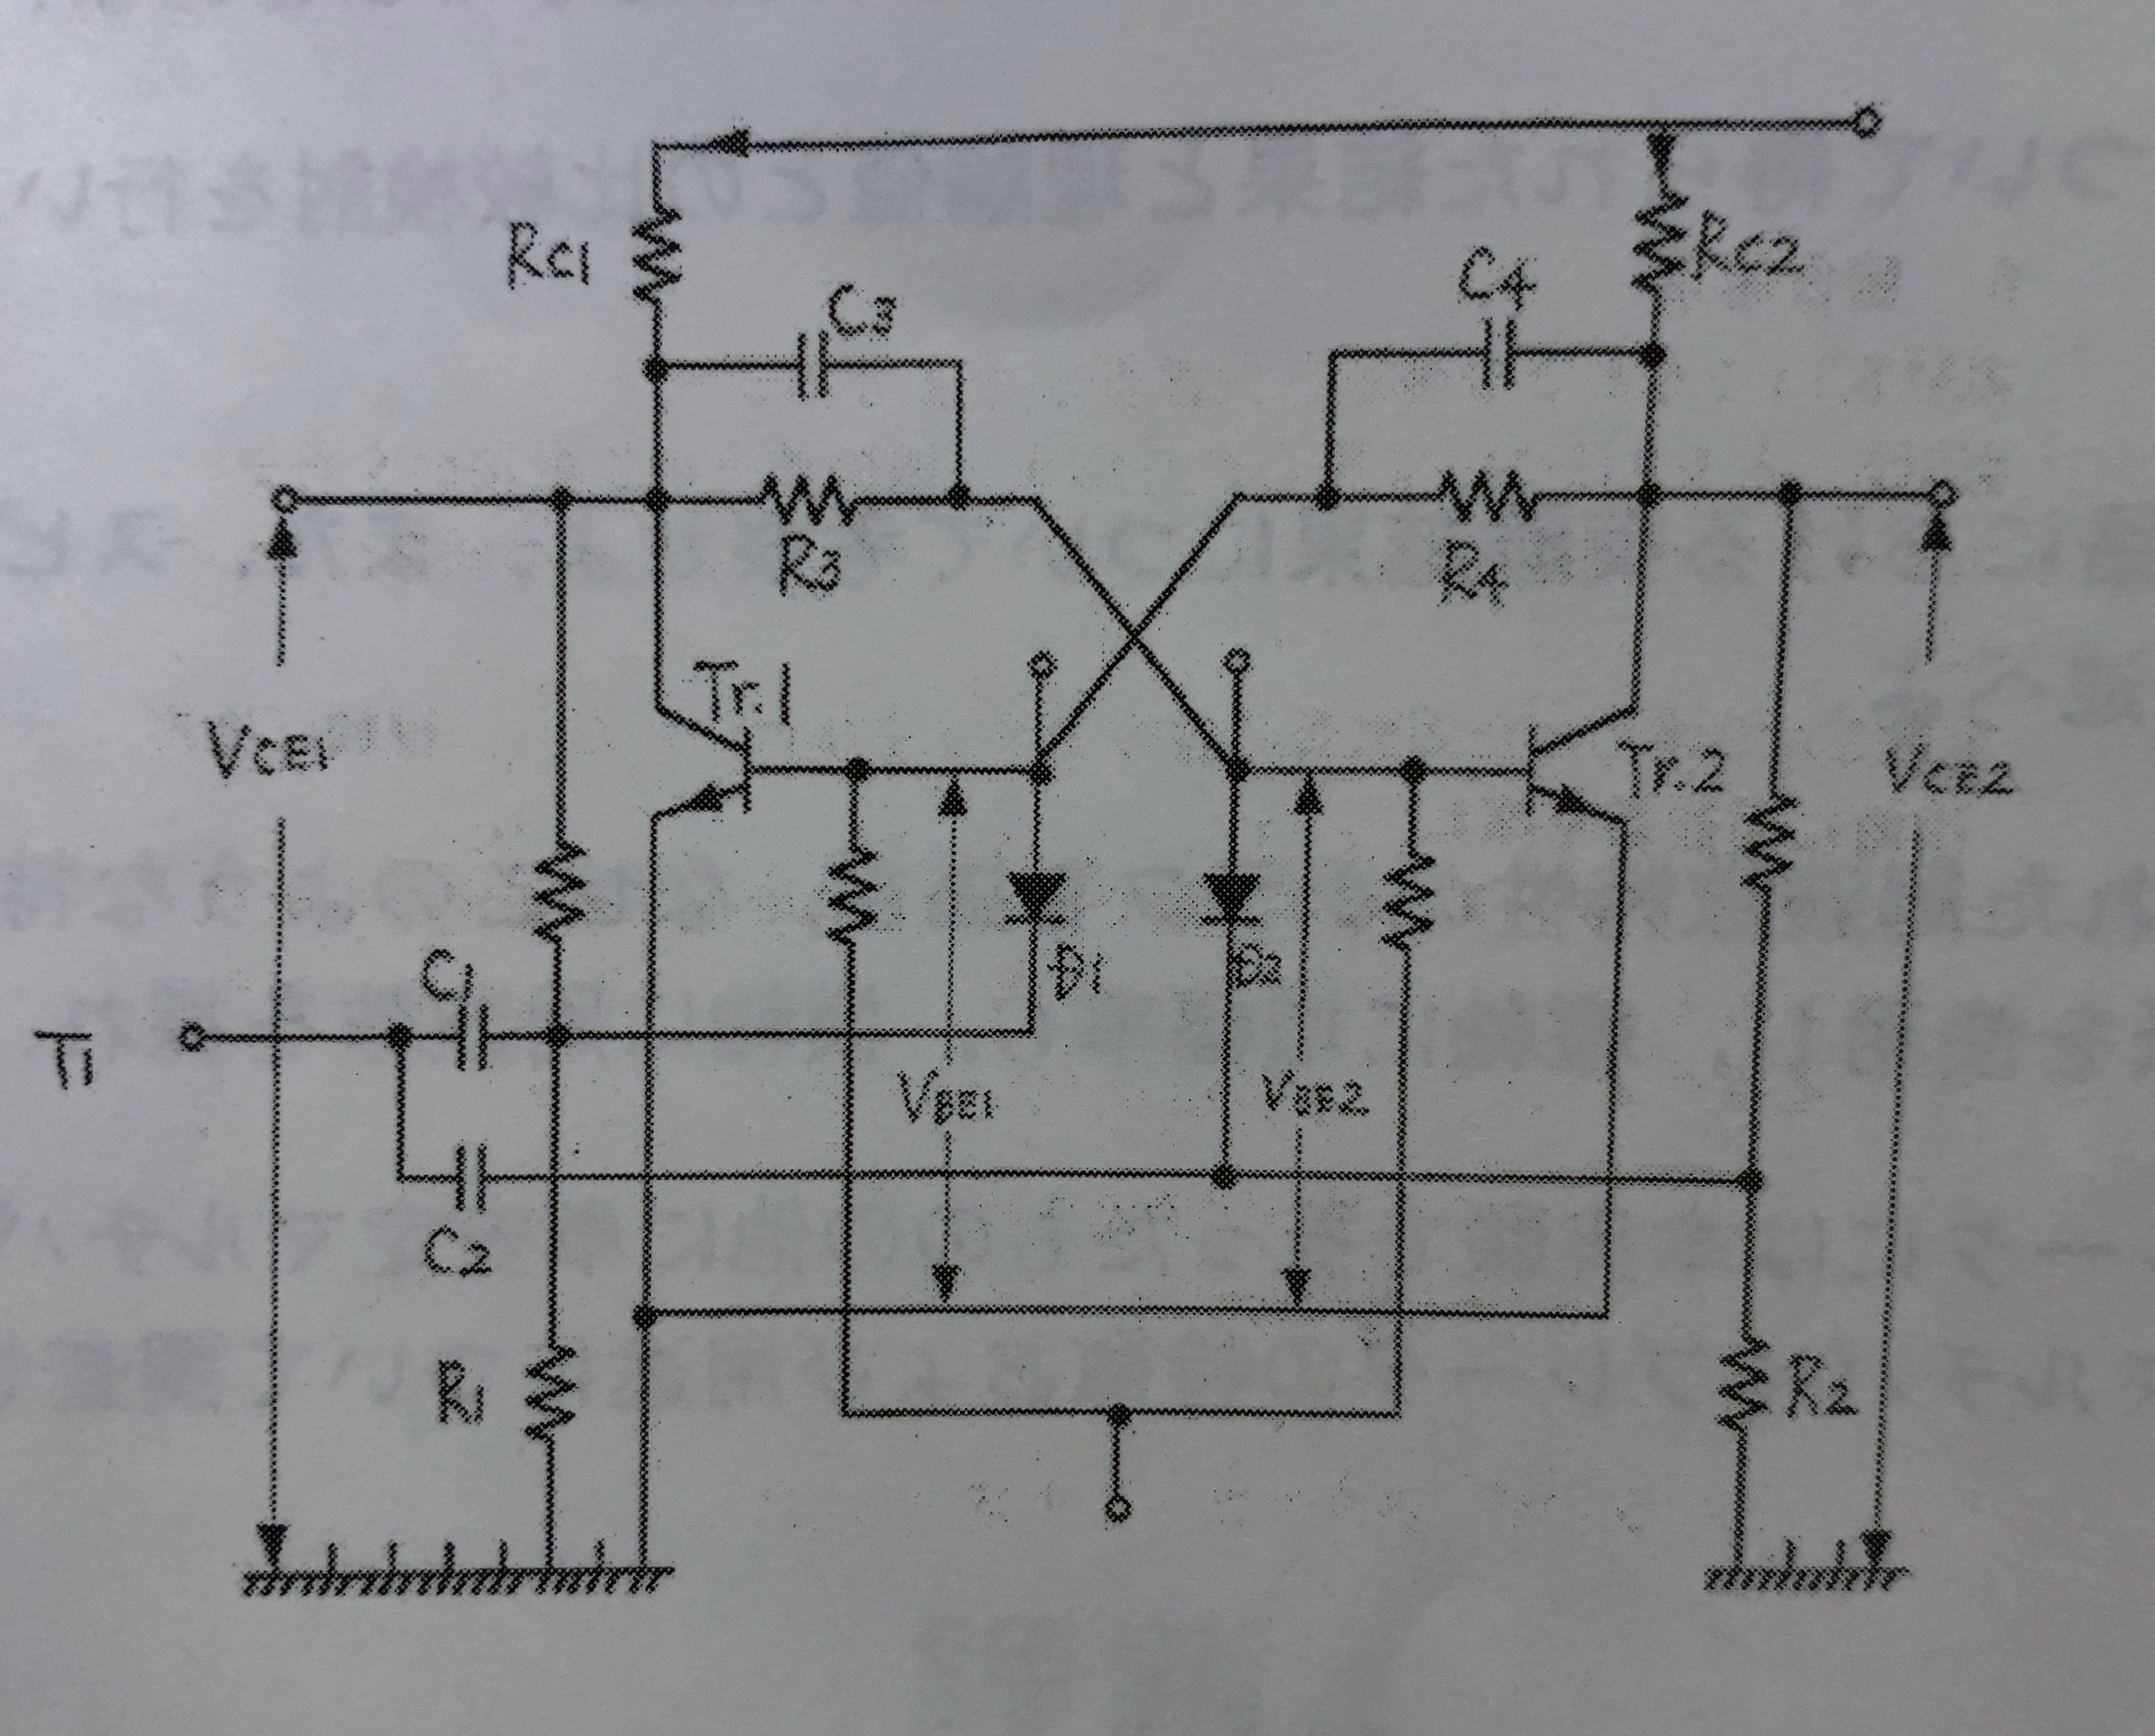
\includegraphics[bb=0 0 2945 2373,height=11cm]{parusu_7.jpg}
    \end{center}
    \caption{双安定マルチバイブレータ}
    \label{fig7}
    \begin{center}
        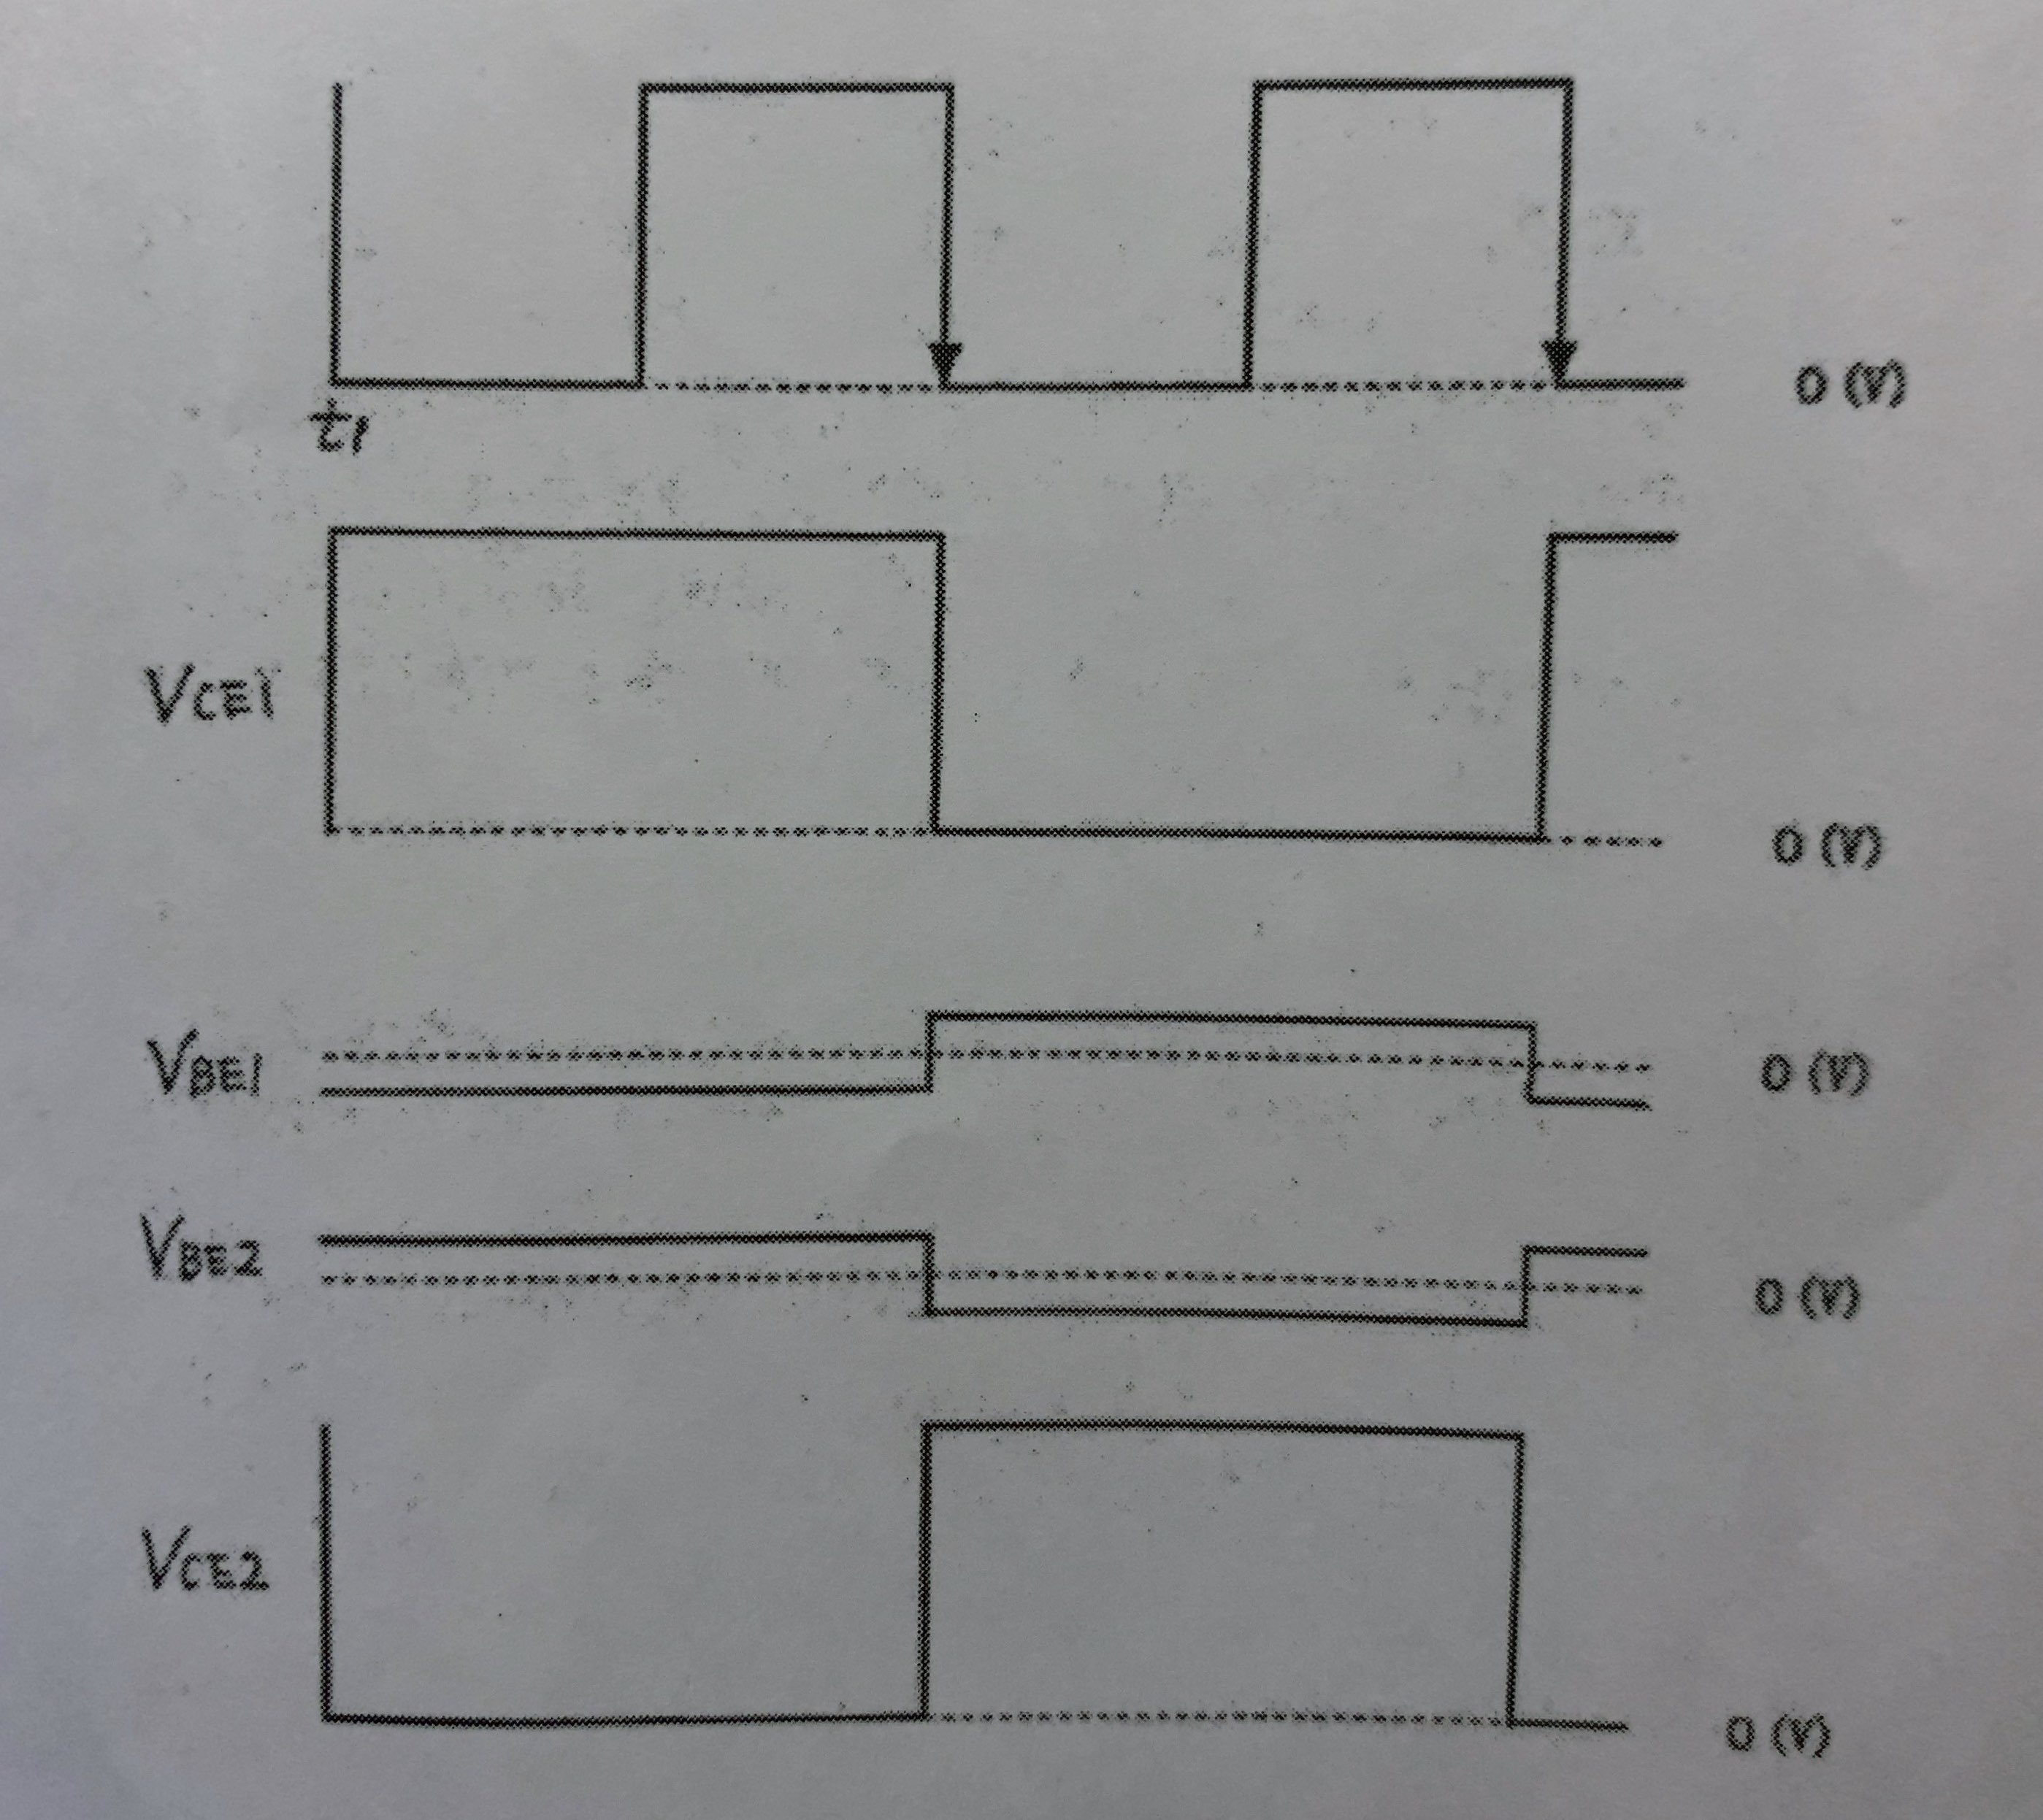
\includegraphics[bb=0 0 2798 2493,height=11cm]{parusu_8.jpg}
    \end{center}
    \caption{双安定マルチバイブレータ 各部の波形図}
    \label{fig8}
\end{figure}
\clearpage

\section{検討・考察}

\subsection{レポート課題1}
\begin{shadebox}
    テキスト中の図3.29は微分回路を示している。
    この回路では入力信号$e(t)$を印加したときに、
    $R$の両側で観測される電圧が$v(t)$であるとき、
    $v(t)$の近似値は$e(t)$を微分した量で与えられる。
    その根拠について考察せよ。
\end{shadebox}
コンデンサにかかる電圧を$V_C(t)$として電流を$i$として、
与えられた文字(抵抗の電圧$v(t)$と入力信号$e(t)$)を用いる。

まず、コンデンサにかかる電圧$V_C(t)$と抵抗の電圧$v(t)$は、
次式(4)、(5)のように表せる。
\begin{eqnarray}
    V_C(t)&=&\frac{\int idt}{C}\\
    v(t)&=&Ri
\end{eqnarray}
キルヒホッフの法則より
\begin{eqnarray}
    e(t)&=&v(t)+V_C(t)
\end{eqnarray}
したがって、式(4)、(5)を代入して、
\begin{eqnarray}
    e(t)&=&Ri+\frac{\int idt}{C}
\end{eqnarray}
式(7)の両辺を$t$で微分すると、
\begin{eqnarray}
    0&=&R\frac{di}{dt}+\frac{i}{C}
\end{eqnarray}
そして、定数分離して微分方程式を解きやすい形にすると、
\begin{eqnarray}
    \frac{1}{i}\frac{di}{dt}&=&-\frac{1}{CR}
\end{eqnarray}
電流$i$を求めるために式(9)の両辺を$t$で積分すると、
\begin{eqnarray}
    \int \frac{1}{i} \frac{di}{dt}dt&=&\int-\frac{1}{CR}dt \nonumber\\
    \int \frac{1}{i}di&=&-\frac{1}{CR}\int dt \nonumber\\
    log_e|i|&=&-\frac{1}{CR}+X \nonumber\\
    i&=&e^{-\frac{t}{CR}+X} \nonumber\\
    i&=&e^Xe^{-\frac{t}{CR}}(Xは積分定数)
\end{eqnarray}
\clearpage

初期条件「$t=0$のとき、$V_C(t)=0$」なので、
式(6)、(7)より、
\begin{eqnarray}
    「t=0のとき、V_C(t)=0」&\Leftrightarrow& 「t=0のとき、e(t)=v(t)」\nonumber\\
    &\Leftrightarrow&「t=0のとき、e(t)=Ri」\nonumber\\
    &\Leftrightarrow&「t=0のとき、i=\frac{e(t)}{R}」
\end{eqnarray}
である。これを、式(10)に代入して、
\begin{eqnarray}
    \frac{e(t)}{R}&=&e^Xe^{-\frac{0}{CR}}\nonumber\\
    \frac{e(t)}{R}&=&e^X
\end{eqnarray}
となるので、回路を流れる電流$i$は
\begin{eqnarray}
    i&=& \frac{e(t)}{R}e^{-\frac{t}{CR}}
\end{eqnarray}
となる。したがって、抵抗にかかる電圧$v(t)$は
\begin{eqnarray}
    v(t)=Ri=e(t)e^{-\frac{t}{CR}}
\end{eqnarray}
となり、 $v(t)$の近似値は$e(t)$を微分した量で与えられることが分かる。

\subsection{レポート課題2}
\begin{shadebox}
    テキスト中の図3.30は積分回路である。
    1.と同様に入力信号$e(t)$を印加したとき、
    $C$の両側で観測される電圧$v(t)$の近似値は$e(t)$を積分することにより与えられる。
    その根拠について考察せよ。
\end{shadebox}
この課題で扱う回路はレポート課題1の回路において$R$と$C$の位置を替えたものであるから、
今回は抵抗の電圧を$V_R(t)$、コンデンサにかかる電圧を$V_C(t)$とすると、
レポート課題1の式(4)、(5)は次のように変形できる。
\begin{eqnarray}
    v(t)&=&\frac{\int idt}{C}\\
    V_R(t)&=&Ri
\end{eqnarray}
この後は、レポート課題1の式(6)~(13)のように同様にして、$i$を導くと、
\begin{eqnarray}
    i&=& \frac{e(t)}{R}e^{-\frac{t}{CR}}
\end{eqnarray}
となるので、$v(t)$は
\begin{eqnarray}
    v(t)&=&\frac{\int e(t)e^{-\frac{t}{CR}}dt}{CR}\nonumber
\end{eqnarray}
となり、$v(t)$の近似値は$e(t)$を積分することにより与えられることが分かる。

\clearpage

\subsection{レポート課題3}
\begin{shadebox}
    スイッチング回路における実験結果について考察せよ。
    また、スピードアップコンデンサの効果について述べよ。
\end{shadebox}
\subsubsection*{スピードアップコンデンサ無し}
スピードアップコンデンサ無しでトランジスタを使用すると応答時間が遅れてしまうので、
ONにしたとき、遅延によって高速なスイッチングはできない。
また、OFFにしたときは、トランジスタが飽和することにより、
ベースに蓄えられる電荷も加わるため、更に遅くなる。

\subsubsection*{スピードアップコンデンサ有り(スピードアップコンデンサの効果)}
電源をONにするとき、入力電圧が上昇するので、
トランジスタのベースには、スピードアップコンデンサを経由した電流が流れて充電される。
変位電流は、電位差が時間的に変化しているときだけ流れるので、
トランジスタが充電された後は変化量がないので、
電位は等しく、ベースへは抵抗を経由してのみ流れる。
電源をOFFにするとき、
ベースはスピードアップコンデンサに蓄えられていた電荷により負電圧がかかり、逆バイアスされる。
よって電源は速やかにOFFになる。
これらのことから、スピードアップコンデンサはスイッチを切り替えた時の反応速度を
上げる効果がある。

\subsection{レポート課題4}
\begin{shadebox}
    本実験では無安定マルチバイブレータ、
    双安定マルチバイブレータを扱っているが、
    これはトランジスタのスイッチング機能を利用している。
    一方、トランジスタにはスイッチング機能の他に信号増幅作用の機能も有している。
    また、トランジスタにはそれぞれに特性曲線が与えられるが、
    これと上記二つの機能との関連について考察せよ。
\end{shadebox}
図\ref{fig9}に示す$I_B=0$の領域を遮断領域、
$V_{CE(S)}$の領域を飽和領域、
点$A$から$B$の領域を入力($I_B$)と出力$(I_C)$が比例関係にあることから、
線形領域または活性領域と呼ばれるが、
この領域内で増幅作用が行われる。
\begin{figure}[h]
    \begin{center}
        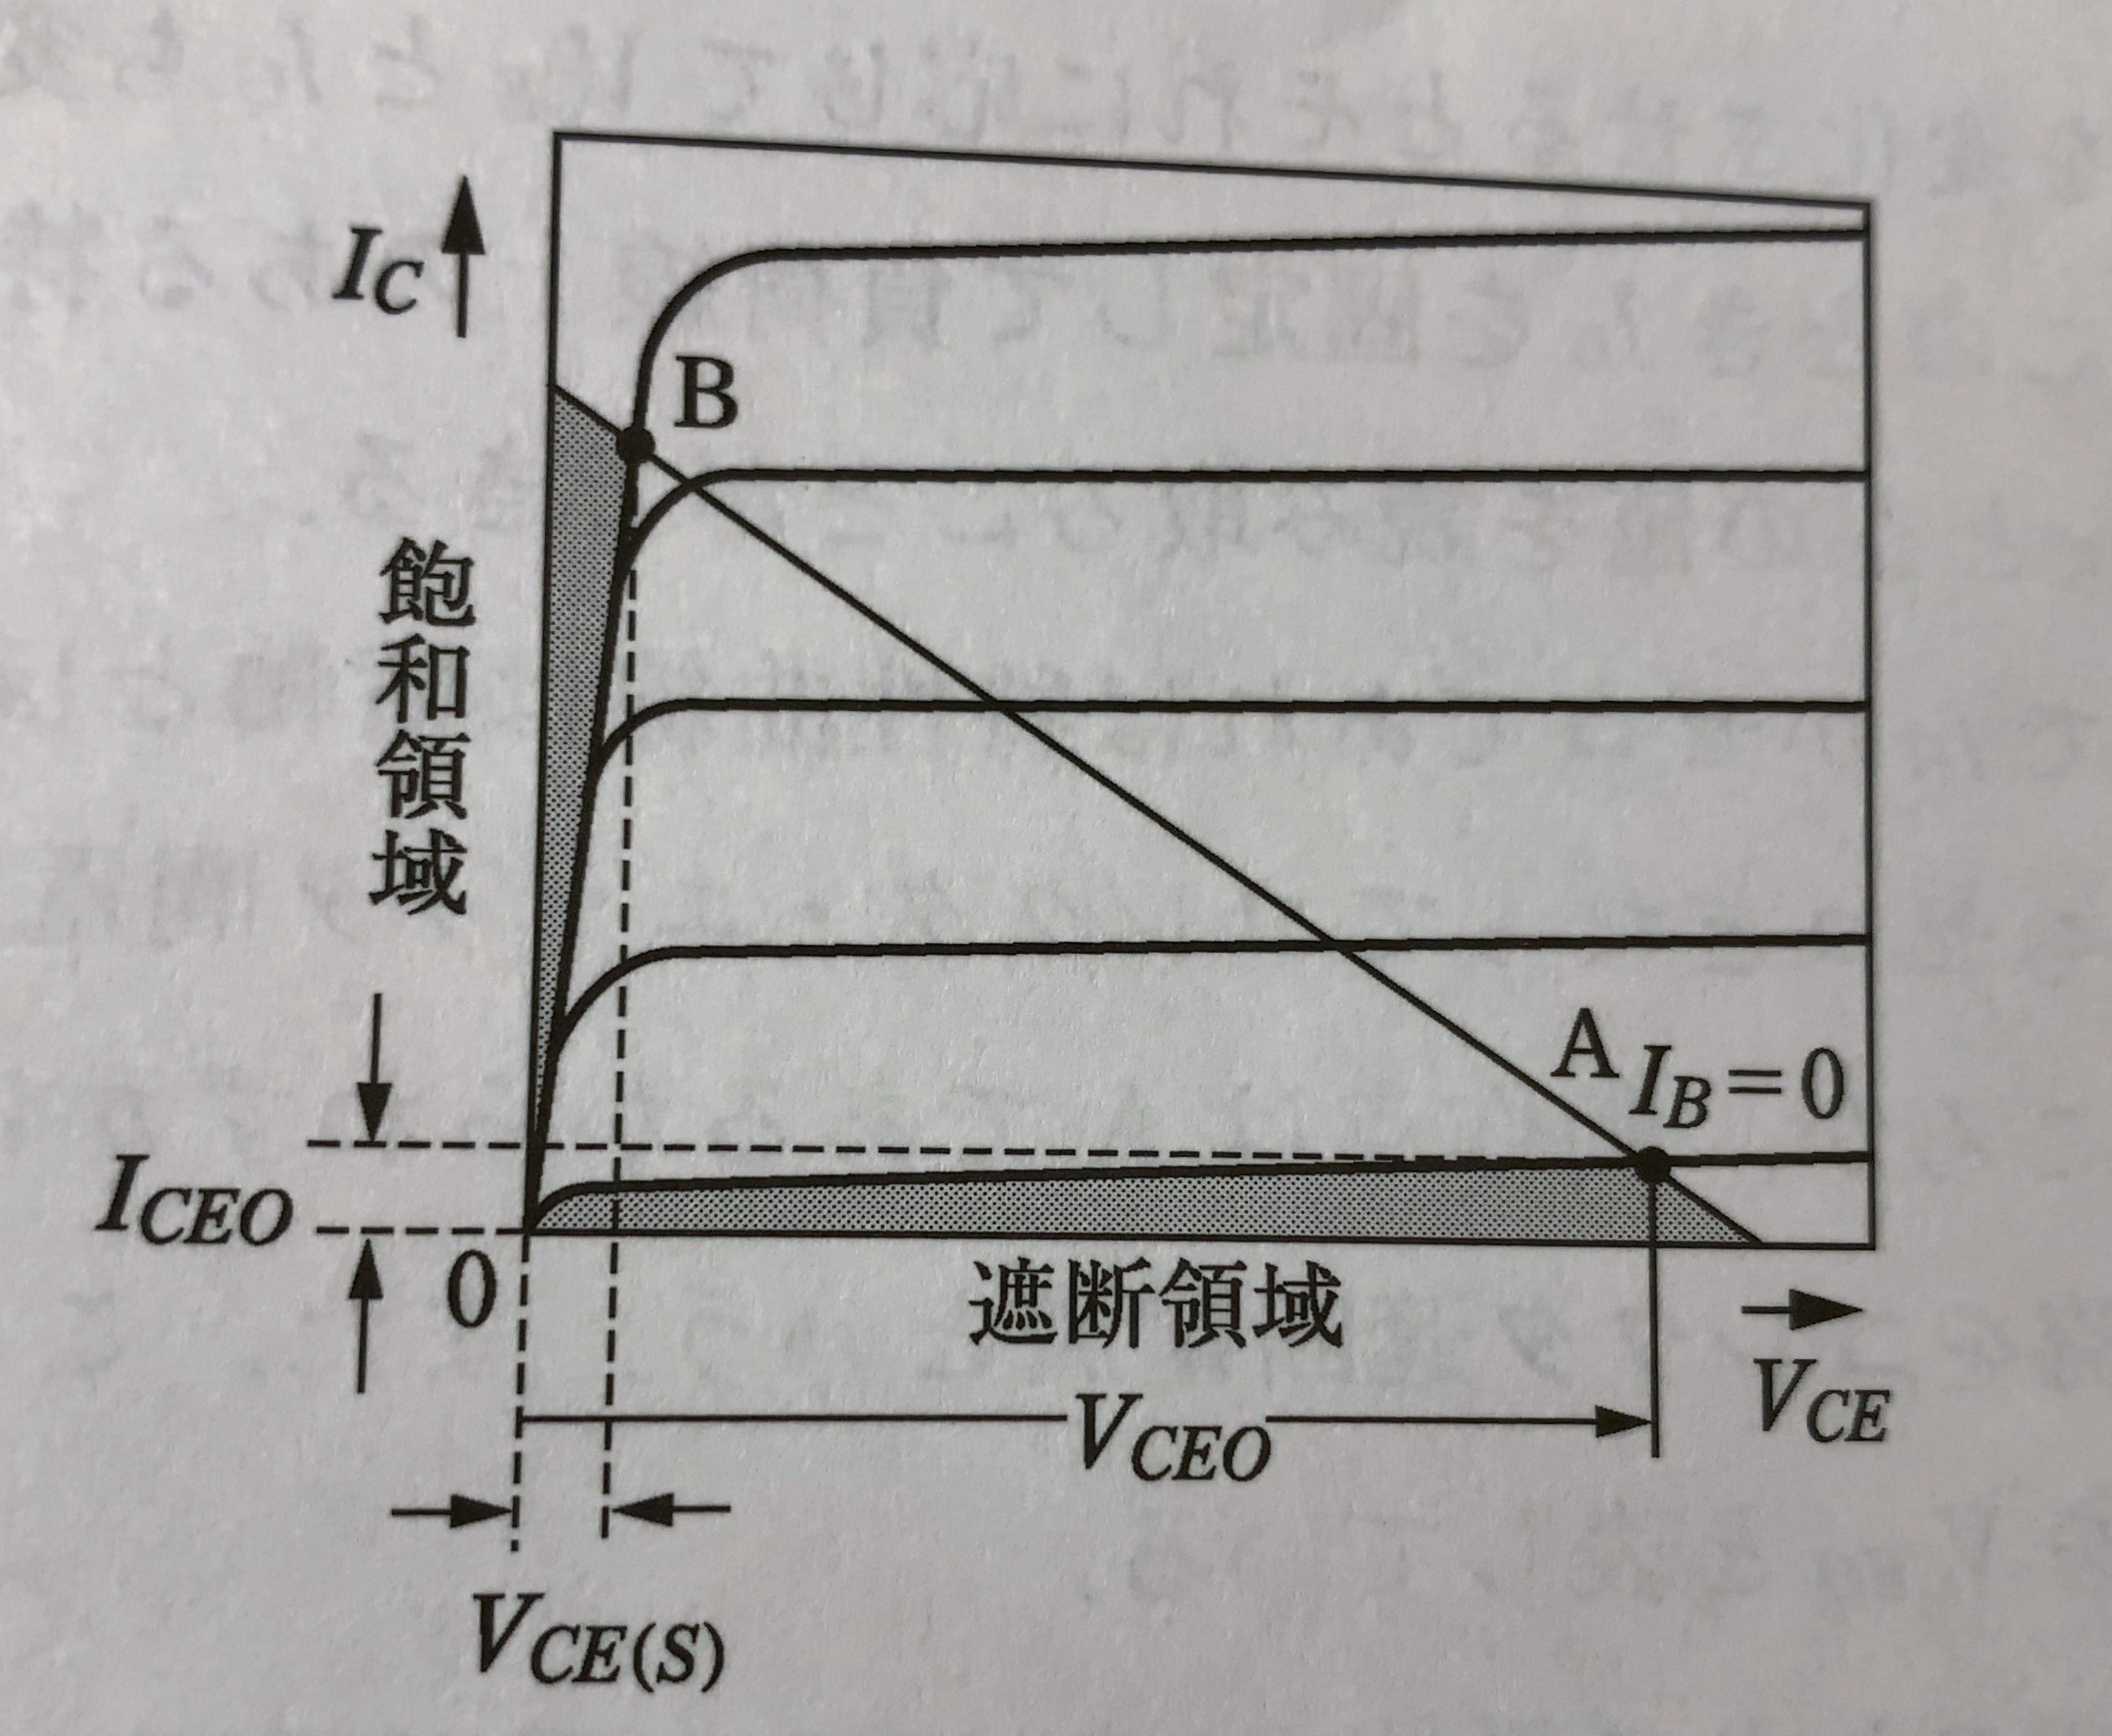
\includegraphics[bb=0 0 2589 2128,height=5cm]{parusu_9.jpg}
    \end{center}
    \caption{トランジスタの動作領域(参考文献7より)}
    \label{fig9}
\end{figure}

ここで、近似的に$I_{CEO} \fallingdotseq 0$、
$V_{CE(S)} \fallingdotseq 0$と考えると、トランジスタのスイッチング作用が分かる。
トランジスタのベース電流をゼロとしたとき、
コレクタ遮断電流$I_{CEO}$がごくわずか流れるが、この電流を無視すれば
動作は動作点は図\ref{fig10}に示す点$A$で、
トランジスタをスイッチに置き換えればOFF状態と考えることができ、
ベース電流を充分大きくするとコレクタ電流は飽和して、
コレクタ・エミッタの電圧$V_{CE(S)}$を無視すれば動作点は図\ref{fig11}の
$B$点で、トランジスタをスイッチに置き換えればON状態と考えられる。

\begin{figure}[h]
    \begin{center}
        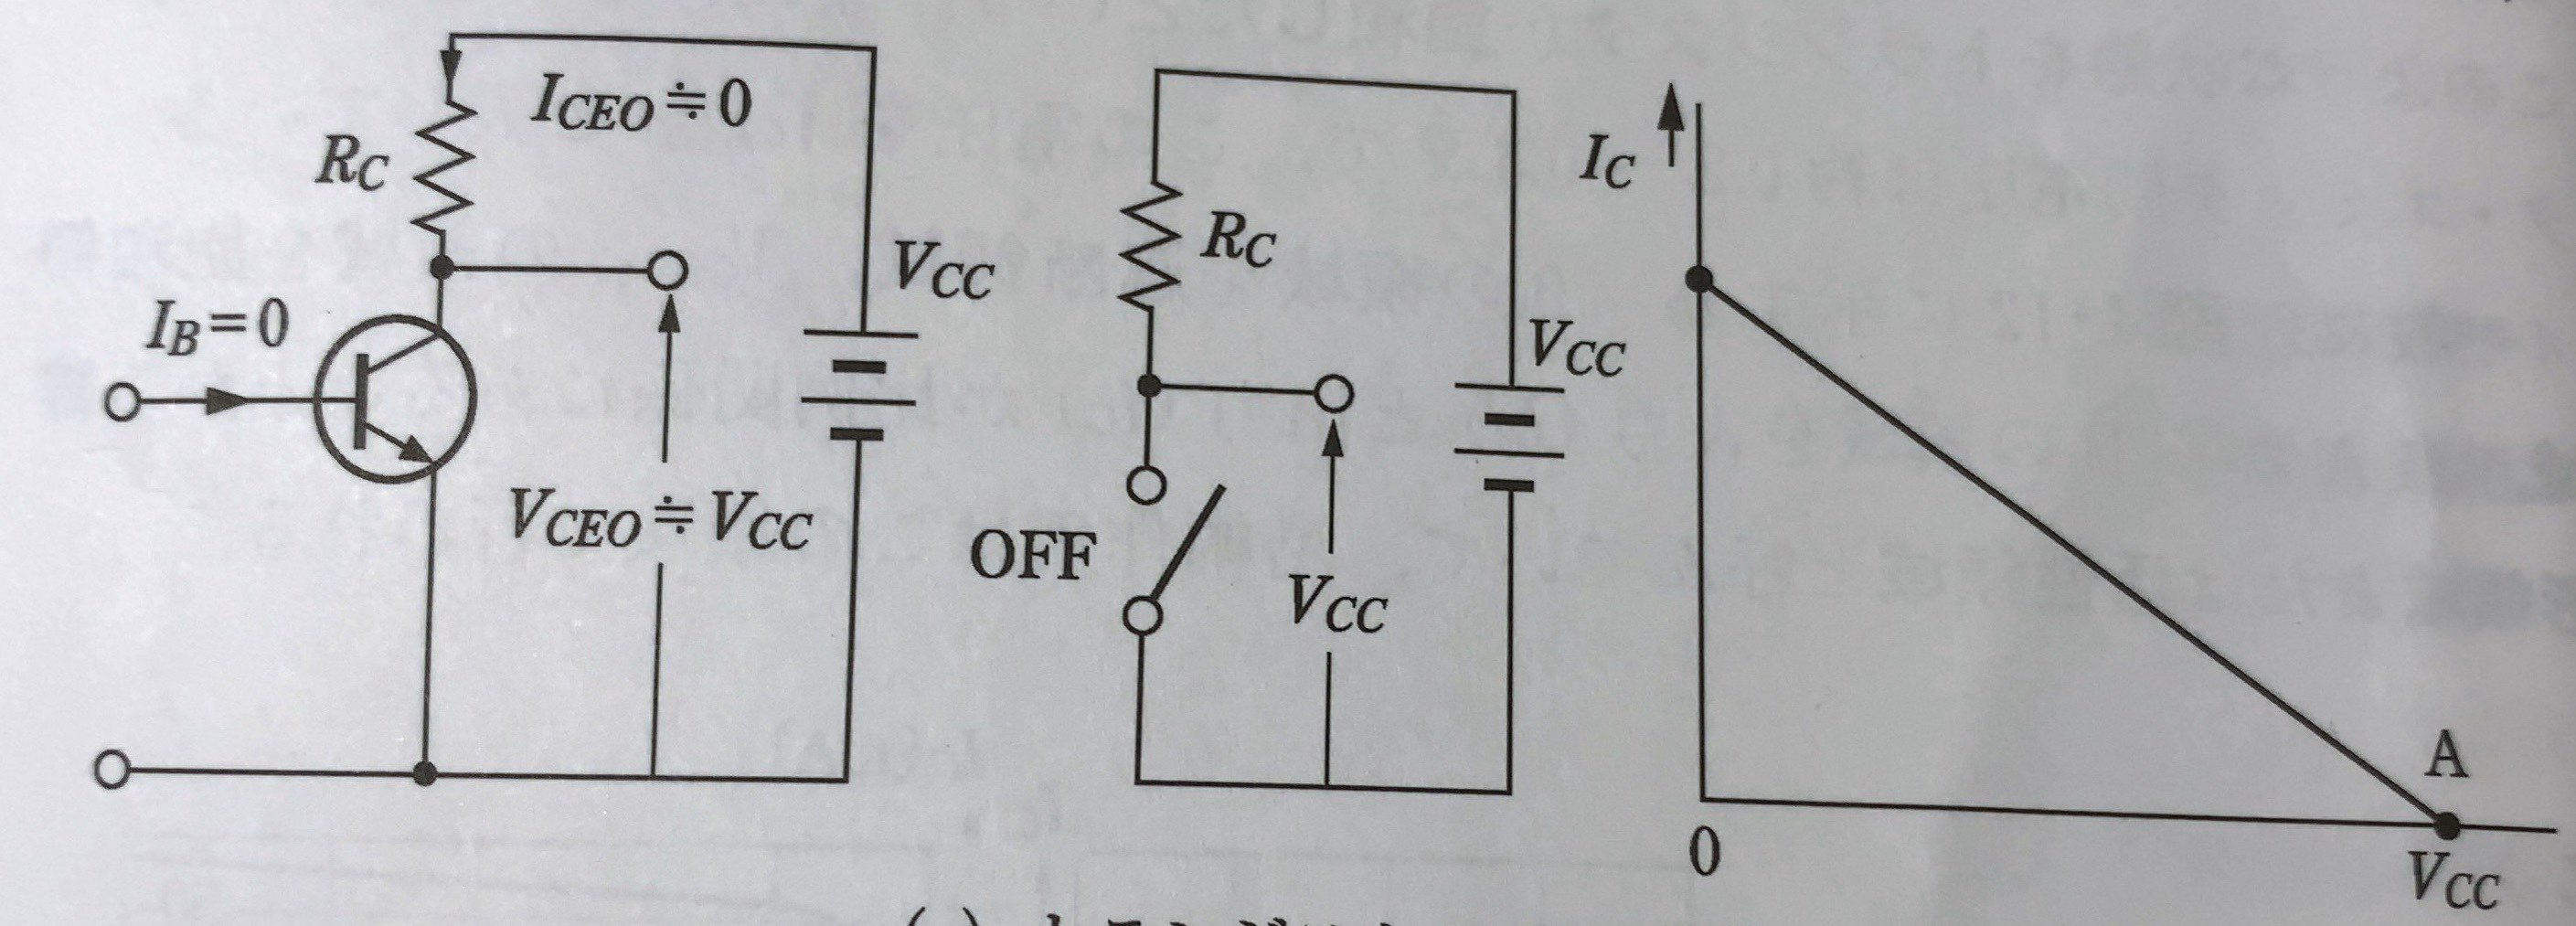
\includegraphics[bb=0 0 2818 1013,height=6cm]{parusu_10.jpg}
    \end{center}
    \caption{トランジスタのOFFの状態(参考文献7より)}
    \label{fig10}
\end{figure}
\begin{figure}[h]
    \begin{center}
        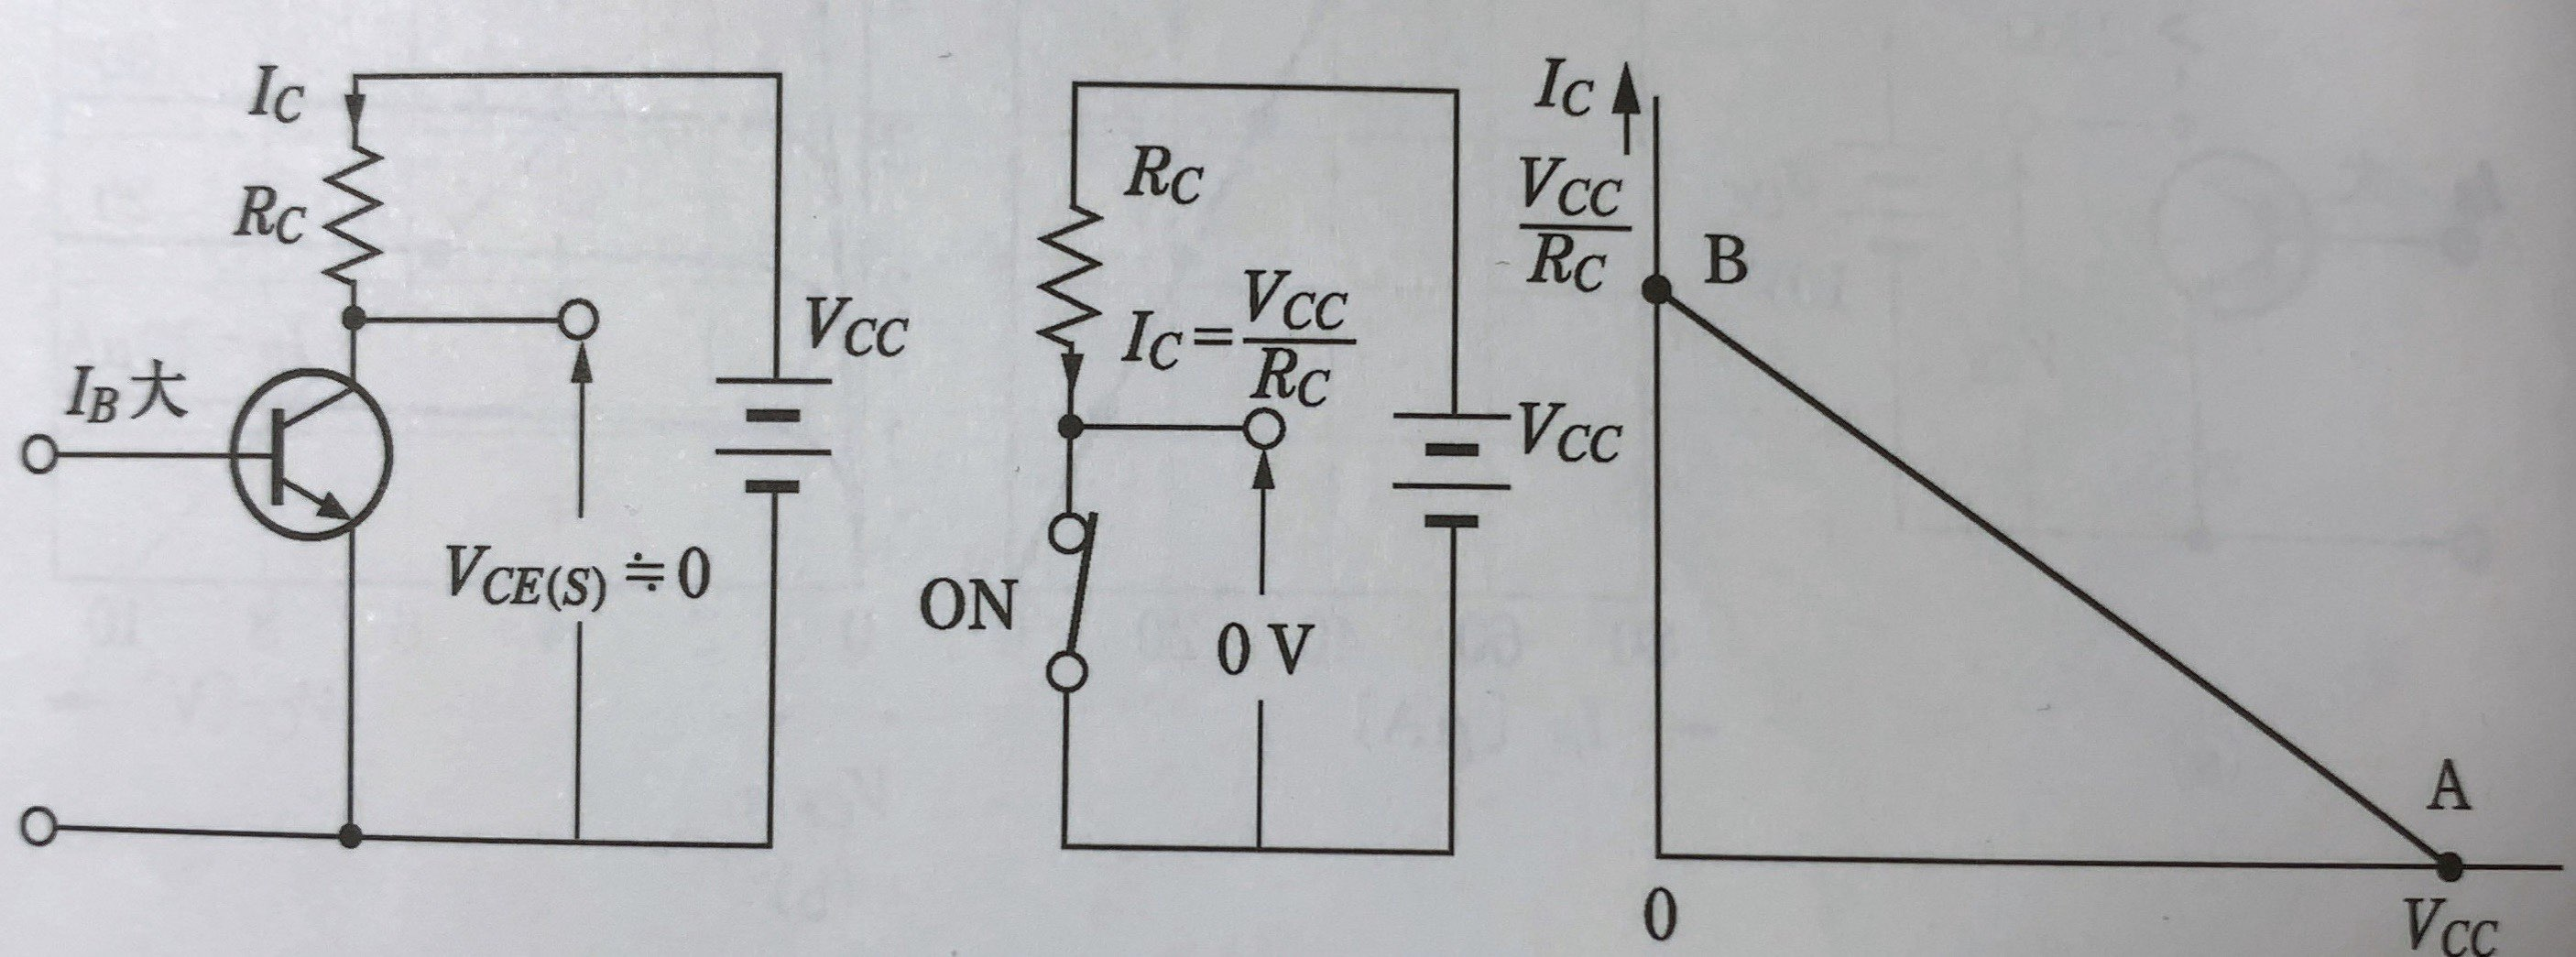
\includegraphics[bb=0 0 2812 1045,height=6cm]{parusu_11.jpg}
    \end{center}
    \caption{トランジスタのONの状態(参考文献7より)}
    \label{fig11}
\end{figure}

\clearpage
\subsection{レポート課題5}
\begin{shadebox}
    マルチバイブレータには本実験で扱ったものの他に単安定マルチバイブレータがある。
    これを含めた各マルチバイブレータの特徴および用途について述べよ。
\end{shadebox}
\subsubsection*{マルチバイブレータの特徴}
\begin{itemize}
    \item 無安定マルチバイブレータ
          \begin{itemize}
              \item 電源をいれると、連続してパルスを発生する。
              \item 2つの状態を常に行ったり来たりすることで発振する。
              \item その周波数は$R$と$C$の値によって決まる。$\frac{1}{CR}$に比例する。
          \end{itemize}
    \item 双安定マルチバイブレータ
          \begin{itemize}
              \item どちらの状態も安定している状態。
              \item 入力2発に対して出力1発が出る。
          \end{itemize}
    \item 単安定マルチバイブレータ
          \begin{itemize}
              \item 一方の状態は安定しているが、もう一方は安定しない状態。
              \item 入力パルスがあると、その波形に無関係に一定波形を出力する。
          \end{itemize}
\end{itemize}
\subsubsection*{マルチバイブレータの用途}
\begin{itemize}
    \item 無安定マルチバイブレータ
          \begin{itemize}
              \item 方形派パルスの発振器
              \item 自動車のウインカーの点滅
          \end{itemize}
    \item 双安定マルチバイブレータ
          \begin{itemize}
              \item 一定幅のパルスを作る
              \item チャタリング防止
          \end{itemize}
    \item 単安定マルチバイブレータ
          \begin{itemize}
              \item コンピュータの記憶回路
          \end{itemize}
\end{itemize}

\section{結論}
パルス回路の動作、原理、特性を動画とテキストにより理解し、パルス技術の基礎を学び、
スイッチング回路やマルチバイブレータの考察を通して、トランジスタについて詳しく知ることができた。

\clearpage
% 参考文献
\begin{thebibliography}{99}
    \label{sannkoubunnkenn_chapter}
    \bibitem[1]{rikadai}東京理科大学工学部情報工学科「情報工学実験1 2020年度」
    (2020/4/6)

    \bibitem[2]{cr_kairo}【CR回路】微分回路の波形・式・原理  |  西住工房

    \url{https://algorithm.joho.info/denki-denshi/cr-kairo-bibun-hakei-shiki-genri/#toc1}

    最終閲覧日:2020/6/23

\end{thebibliography}

\clearpage
\appendix
%%%%%%%%%%%%%%%%%%%%%%%%%%%%%%%%%%%%%%%%%%%%%%%%%%%%%%%
\end{document}
